\setlength{\parindent}{2em} %首行缩进

\section{實驗目的:}
\begin{enumerate}[label=\arabic*.]
  \item 利用 PCR 技術,複製大腸桿菌轉型實驗中的DNA。
  \item 觀察並比較轉型成功與未成功的細菌 DNA 電泳結果。

\end{enumerate}



\section{實驗步驟:}

\subsection*{實驗器材}

\begin{multicols}{2}
  \begin{enumerate}[label=\arabic*.]
    \item polymerase reagent(20μL)
    \item primer mixture(20μL)
    \item 大腸桿菌轉形實驗中含藍、白菌落的培養基
    \item 500μL 的 PCR tube x2
    \item P20
    \item Eppendorf
    \item PCR machine
    \item 電泳儀
    \item 電源供應器
    \item Agarose gel
    \item 電泳 buffer
    \item Light box
    \item 離心機
  
  \end{enumerate}  
\end{multicols}

\subsection*{步驟}

\begin{enumerate}[label=\arabic*.]
  \item 取兩個 500μL 的 PCR tube 並用標示 W 和 B,各自加入 10μL 的 polymerase reagent 和 10μL 的 primer mixture,再pipetting 得到 PCR sample。
  \item 用兩個 P200/P20 的 tip 分別沾取培養基中的藍色與白色菌落,再分別加入標示 W 和 B 的 PCR tube,與 PCR sample 均勻混合。(若混合後氣泡過多或液體殘留在管壁,可先離心再進行下一步驟)
  \item 將標示 W 和 B 的 PCR tube 放到 PCR machine 中反應 40 分鐘。
  \item 從 W 和 B 兩管各用 pipette 取 10μL 到 eppendorf 的蓋子上,再分別取 2μL 的 loading buffer 與之混合,最後 load 到 agarose gel 裡面,以 140V 電泳 15 分鐘。
  \item 將跑完的 agarose gel 放到 light box 觀察。
  
\end{enumerate}



\newpage
\section*{實驗結果及討論:}
\subsection*{結果}
\begin{figure}[H]
\centering
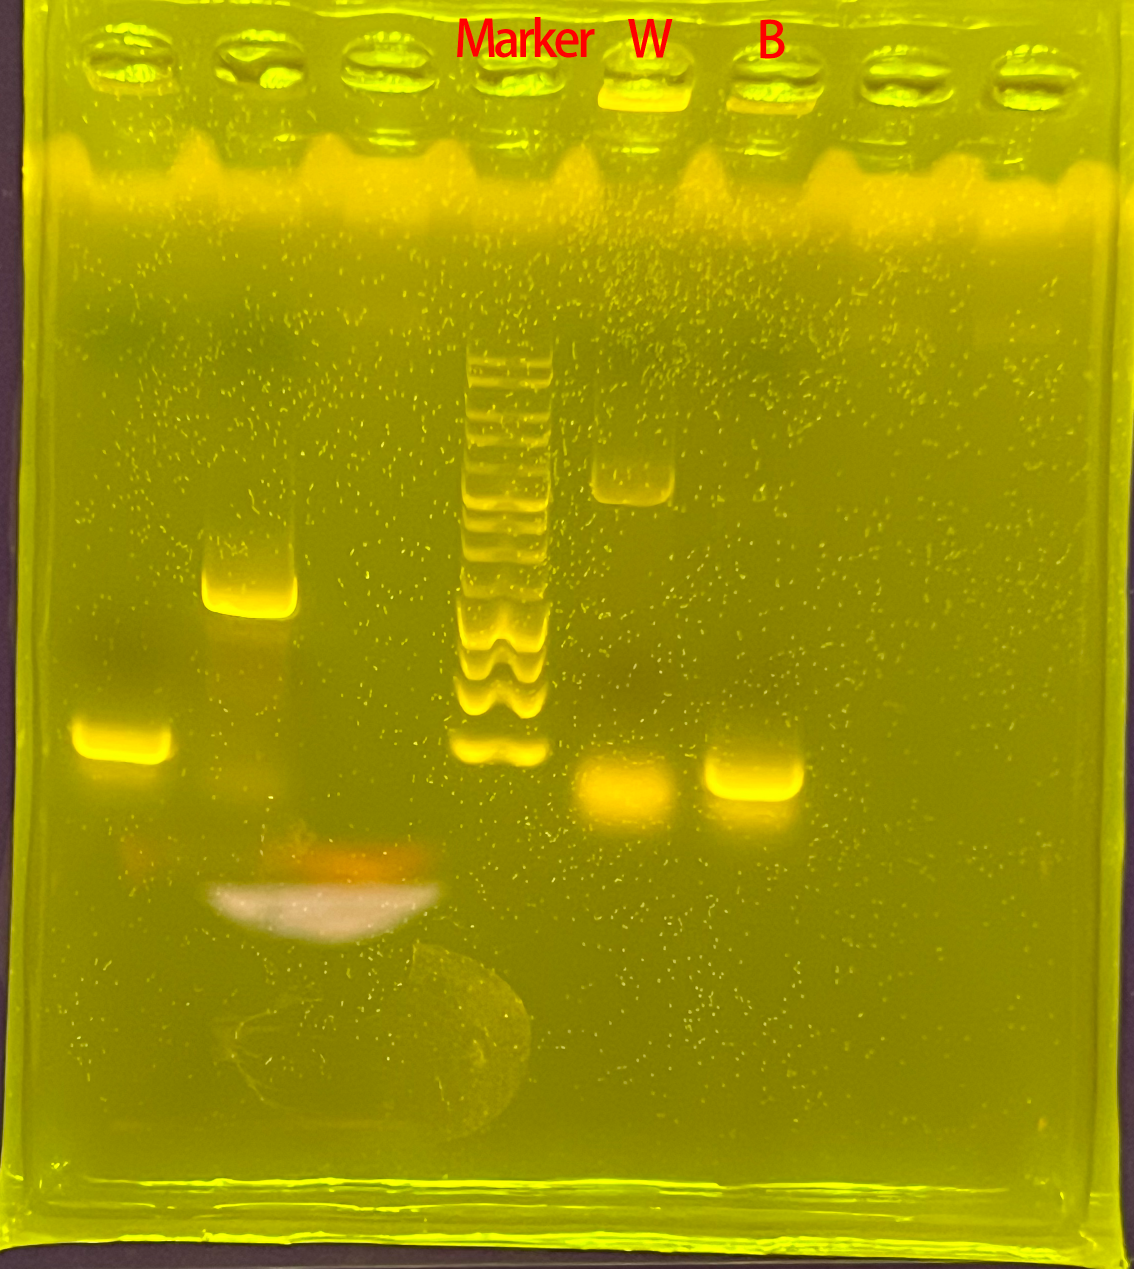
\includegraphics[width=0.5\textwidth]{paste_src/rt1.png}
\end{figure}

\begin{enumerate}[label=\arabic*.]
  \item 白色菌落 (W組) 在 3-4kbp 與有明顯亮帶,於 250bp 以下有較模糊的亮帶。
  \item 藍色菌落 (B組) 僅在 250bp 以下有明顯亮帶。
\end{enumerate}


\subsection*{實驗討論}


\dsc 電泳結果的意義 
\begin{enumerate}[label=\arabic*.]
  \item 白色菌落的 colony 有成功 insert,其 DNA 分子量較大,電泳時移動速度較慢;藍色菌落的 colony 未成功 insert,其 DNA 分子量較小,電泳時移動速度較快。
  \item 白色菌落在對藍色菌落的亮帶處也有模糊的亮帶,推測是因為沾取到部分沒有 insert 成功的 colony 造成。
  \item 藍色與白色菌落的 colony 皆為環狀 DNA ,其分子量都比對應到的 Marker 分子量大。

\end{enumerate}


\newpage

\dsc Real-time PCR介紹

\begin{itemize}[leftmargin=0cm,]
  \item[] 目的:除了PCR增加目標片段DNA作用,利用螢光物質與DNA片段結合的效果,藉由偵測濃度,達到定量效果。
  \item[] 目前主要分為TaqMan與SYBR green兩種
\end{itemize}

\begin{table}[h]
\centering
\setlength{\abovecaptionskip}{0cm} % 调整caption间距
\begin{tabular}{cp{6cm}p{6cm}}
\toprule
方式&SYBR green&TaqMan\\

\midrule
原理&藉由螢光染劑對雙股DNA有較高親和力的效果,達成PCR過程中螢光強度會隨著cycle數目增加的定量方式。&藉由DNA探針上兩個螢光基團,分別為紅綠,當兩基團較接近時,紅色螢光因為波長較長造成綠色螢光無法被偵測,而PCR過程中,兩基團隨著DNA合成而遠離,綠色螢光基團則可被偵測,達成定量目的。\\
\midrule
優點&較便宜、降低實驗設計的複雜度&較為準確\\
\midrule
缺點&比起TaqMan方式有較高的誤差&設計DNA探針較為複雜、昂貴\\
\bottomrule


\end{tabular}\end{table}





%\bibliography{bibfile} 
%\bibliographystyle{unsrt}
